\Titre{Arduino Security}

\begin{document}

\begin{reveals}
		
\maketitle


\section{Arduino}

\begin{frame}[c]{Presentation}
  
  \begin{block}{Micro-controller}
    \begin{itemize}
    \item AVR ATMega micro-controller
    \item ``Harvard'' architecture
    \item 8 bits native, 16 bits operations
    \end{itemize}
  \end{block}

  \vfill

  \begin{block}{Board}
    In addition to a controller:
    \begin{itemize}
    \item Power and USB
    \item (Lot of) PINs to communicate with \emph{sensors} and
      \emph{actuators}
    \end{itemize}
  \end{block}
  \vfill

  \begin{block}{Applications}
    \begin{itemize}
    \item Basis for robotics, IoT, etc.
    \item Teaching embedded systems programming
    \item Fast \& easy prototyping
    \item Ideal for low-cost DIY projects
      \begin{center}
        \color{red}high-end alternative: Raspberry \(\pi\)
      \end{center}
    \end{itemize}
  \end{block}

\end{frame}


\section{Physical Security Analysis}


% Missing: the USB controller

\fullimage{images/Arduino-Uno-board-pins-description.jpg}


\begin{frame}
  \frametitle{Physical Security Analysis}

  \begin{enumerate}[<+->]
  \item List the physical areas and the possible communication
    channels
    \begin{center}
      \fbox{~~\begin{minipage}{.8\linewidth} Goal is to list
          communication channels with the internal of
          the \(\mu\)-controller when having access to the board
      \end{minipage}~~}
    \textcolor{red}{\(=\) Attack surface}
    \end{center}
  \item Assess the expertise needed to actually use each of these channels
    \begin{center}
      \fbox{~~\begin{minipage}{.8\linewidth}
        Goal is to determine who can do what
      \end{minipage}~~}
    \end{center}
  \item Describe the attack surface without connecting directly to the
    PINs of the controllers
      \fbox{~~\begin{minipage}{.8\linewidth} 
          Good compromise, most circuitry is electronics, not security
      \end{minipage}~~}
  \end{enumerate}

\end{frame}
\begin{comment}
  At the end of this exercice, the attack surface is:
  \begin{itemize}
  \item connection to I/O pins
  \item connection to USB
  \item connection to ICSP (In-Circuitry Serial Programming)
  \end{itemize}

\end{comment}

\fullimage{images/arduino-pinout-complete.png}

\fullimage{images/arduino-pinout-summary.png}



\begin{frame}{I/O Pins}
  
  \begin{block}{Most cases}
    \begin{itemize}
    \item Can only retrieve or enter data
    \item RX/TX (reception/transmission): UART protocol (for
      communication with a computer)
    \item MISO/MOSI/SCLK/NSS: SPI protocol, fast, but needs 4 pins
    \item SDA/SCL: I2C protocol, 2 pins needed for communication with
      a sensor/actuator or another Arduino
    \item Pins are linked to registers in the \(\mu\)-controller
    \item Analysis of the program in the \(\mu\)-controller:
      \begin{itemize}
      \item Check what is done with data received (read on registers)
      \item Check what data is sent on the pins (written on registers)
      \end{itemize}
    \end{itemize}
  \end{block}

  \vfill

  \begin{block}{Parallel Programming}
    \begin{itemize}
    \item A special mode in which both the serial bus controller and
      the ATMega328 \(\mu\)-controller can be written
    \item More details later
    \end{itemize}
  \end{block}

\end{frame}

\begin{frame}[c]{USB connector}
  
  \begin{block}{Most cases}
    \begin{itemize}
    \item Is actually employed to upload programs on the ATMega328
      \(\mu\)-controller
    \item Controlled by the ATMega16U2 controller (USB interface), as
      well as the previous I2C and UART protocols
    \end{itemize}
  \end{block}

  \vfill

  \begin{block}{Keyboard and Mouse}
    \begin{itemize}
    \item The USB controller may pose as being connected to several
      USB devices
    \item Including a Mouse and a Keyboard in the standard library
    \item In that case it can send keyboard and mouse events
    \item This is used in rogue USB devices (\textit{e.g.} USB keys)
      to penetrate a system
    \end{itemize}
  \end{block}

\end{frame}

\begin{frame}{In-Circuitry Serial Programming}
  
  \begin{block}{Usage}
    \begin{itemize}
    \item Update to the serial controller \textcolor{red}{and} the
      ATMega328 \(\mu\)-controller
    \item These updates \textcolor{red}{cannot} be controlled
    \item As in Parallel Programming, these updates start with erasing
      all the memory
    \end{itemize}
  \end{block}

  \vfill

  \begin{block}{Security Analysis}
    \begin{itemize}
    \item Availability: can be ensured only if reset disabled
    \item Confidentiality is preserved in case of reset (all bits are
      really set to 1)
    \item Integrity:
      \begin{itemize}
      \item Need to focus on the case of an apparently functioning
        device
      \item Authentication: The device serial number is not sufficient
        to decide we can send information to this device, the program
        may have been replaced with a malware
      \end{itemize}

    \end{itemize}
  \end{block}

\end{frame}


\begin{frame}[c]{Parallel Programming}
  
  \begin{block}{Principle}
    \begin{itemize}
    \item Uses 20 pins for power, data, and control
    \item Faster than serial
    \end{itemize}
  \end{block}

  \vfill

  \begin{block}{Practical Aspect}
    \begin{itemize}
    \item Mostly with a dedicated ``writer'' device set up to program
      other devices
    \item Same comments as for ICSP \textit{re.} capabilities and
      reset
    \end{itemize}
  \end{block}

\end{frame}


\begin{frame}[c]{Summary}
  
  \begin{block}{Security concerns}
    \begin{itemize}
    \item Sensitive data inside the \(\mu\)-controller
      \begin{itemize}
      \item Programs integrity needs to be protected
      \item Data integrity and confidentiality
      \end{itemize}
    \item Attack surface:
      \begin{itemize}
      \item The pins and the USB plug
      \item Information on these pins is either:
        \begin{itemize}
        \item ``passive'', and given as data in registers of the
          \(\mu\)-controller
        \item ``active'', and can reset the \(\mu\)-controller without
          any recourse
        \end{itemize}
      \item In all cases, additional channel: interruptions telling
        that some data is available (\(+\) internal clock
        interruptions)
      \end{itemize}
    \item Next step: look at the internals of the \(\mu\)-controller
      to check the security of programs
    \end{itemize}
  \end{block}

\end{frame}


\section{The ATMEL ATMega328p controller}


\subsection{Memory Model}

\begin{frame}[c]{Harvard Architecture}
  
  \begin{block}{Von Neumann Architecture}
    \begin{itemize}
    \item Unified address space space for data and programs
    \item Most common at the application level
      \begin{center}
        Windows and Unix processes have a unique address space
      \end{center}
    \end{itemize}
  \end{block}

  \vfill

  \begin{block}{Harvard Architecture (ATMega)}
    Three disjoint address spaces:
    \begin{itemize}
    \item Program memory (32kB): program code and constant data
    \item SRAM (2kB): the place where variables' values are stored during
      the execution of programs, including 16bits registers (L/H)
    \item EEPROM (1kB): mostly for flags configuring the processor's
      functions and security
    \item The address \texttt{0x200} corresponds to two different
      bytes, one in the program memory, one in the SRAM
    \end{itemize}
    The address space to be used depends on the instruction (different
    load/store instructions)
  \end{block}

\end{frame}


\begin{frame}[c]{The SRAM}

  \begin{center}
    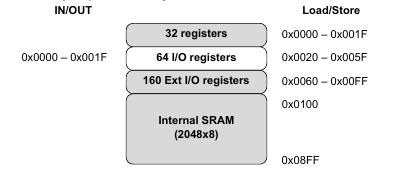
\includegraphics[width=0.8\textwidth]{images/arduino-SRAM.png}
  \end{center}

  \only<1>{
      \begin{block}{32 registers (CBI/SBI and LD/ST)}
        \begin{itemize}
        \item Employed for arithmetic, etc.
        \item They have names
        \item X, Y, Z: used for indirect addressing (functions, table of symbols)
        \end{itemize}
      \end{block}
}
\only<2>{\begin{block}{64 registers (IN/OUT and LD/ST)}
        \begin{itemize}
        \item Those connected to the ``outside''
        \item They have names too
        \item Example: stack pointer is here
        \end{itemize}
      \end{block}
}
\only<3>{
      \begin{block}{Other registers \& memory (LD/ST)}
        \begin{itemize}
        \item Most registers still have names 
        \item Registers for communication protocols are here
        \item Only LD/ST can be used to read/write here
        \item Stack and heap are in the rest of the SRAM
        \end{itemize}
      \end{block}
}
\end{frame}



\begin{frame}[c]{The EEPROM}
  
  \begin{block}{Instructions}
    \begin{itemize}
    \item LD/ST (load/store): take 1 address and 1 byte
    \item LD: copy the byte at that address to the target byte
    \item ST: copy the byte into the target address
    \end{itemize}
  \end{block}
  
  \vfill

  \begin{block}{LD/ST and the address space}
    \begin{itemize}
    \item One 16b register at address \texttt{0x41-0x42} of the SRAM
    \item One 8b register at address \texttt{0x40} of the SRAM
    \item LD/ST with these registers will interact with the EEPROM
      instead of the SRAM
    \end{itemize}
  \end{block}


\end{frame}


\begin{frame}{The Program Memory}
  
  \begin{columns}
    \begin{column}{0.45\textwidth}
      \begin{block}{Description}
        \begin{itemize}
        \item Contains the instructions
        \item Two security levels: Application and BootLoader Space (BLS)
        \item Instructions are read by the processor
        \item Possible communication with the SRAM:
          \begin{itemize}
          \item LPM: Load from address in program memory to address in SRAM
          \item SPM: Store from address in SRAM to address in program memory
          \end{itemize}
        \end{itemize}
      \end{block}
      
    \end{column}

    \begin{column}{0.45\textwidth}
      \begin{center}
        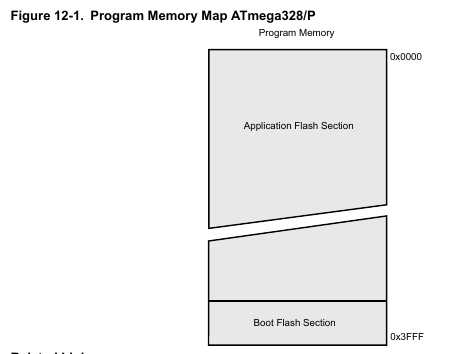
\includegraphics[trim=200 0 20 40 ,clip,height=6cm]{images/arduino-progmem.png}
      \end{center}      
    \end{column}
  \end{columns}


\end{frame}


\begin{frame}[c]{Exercice}
  
  \begin{enumerate}
  \item Make a diagram of the different memory parts, each with the
    communication channels to and from that part
  \item How would you model them in the BLP/Biba models?
  \item What are the subjects and the objects here? What can you say
    on Access Control?
  \end{enumerate}

\end{frame}

\subsection{Memory Security}

\begin{frame}{The LPM/SPM instructions}
  
  \begin{block}{LPM}
    \begin{itemize}
    \item This instruction can appear anywhere in the Program Memory
    \item It is very useful to store strings in the program data,
      before loading them in the memory for further processing
    \item Its behaviour is controlled by lock bits
    \end{itemize}
  \end{block}

  \vfill

  \begin{block}{SPM}
    \begin{itemize}
    \item This instruction can only be in the Boot Flash Section
    \item When seen at an address in the Application Flash Section, it
      is replaced with a NOP
    \item Its behaviour is also controlled by lock bits
    \end{itemize}
  \end{block}

\end{frame}

\definecolor{deepblue}{RGB}{0,0,64}
\begin{frame}[c]{Access Control on Physical Programming}
  
  \begin{center}
    \begin{tabular}{|c|c|c|p{0.6\textwidth}|}
      \arrayrulecolor{deepblue}
      \hline
      \multicolumn 3{|c|}{\cellcolor{deepblue}\textcolor{white}{Memory Lock Bits}}&\multicolumn 1{c|}{\cellcolor{deepblue}}\\[-.1ex]
      \cellcolor{blue!50!black}\textcolor{white}{LB Mode} & \cellcolor{blue!50!black}\textcolor{white}{LB2} &  \cellcolor{blue!50!black}\textcolor{white}{LB1} & \multicolumn 1{c|}{\multirow{-2}{*}{\cellcolor{deepblue}\textcolor{white}{Protection Type}}} \\      
      1&1&1& No memory lock\\      \hline
      2&1&0& No write with Parallel \& Serial Programming\\      \hline
      3&0&0& No read (verification)\&write with Parallel \& Serial Programming\\      \hline
    \end{tabular}
  \end{center}

  \begin{block}{Notes}
    \begin{itemize}
    \item Lock bits are in EEPROM, by default (after reset) the value
      is one, setting a bit means giving it the value 0
    \item The (parallel or serial) programmer can still issue a
      \emph{chip erase} command, that will unset the lock bits
    \item Conclusion: Availability cannot be ensured against physical
      attackers, but confidentiality and integrity can be preserved
      (against programmers)
    \end{itemize}
  \end{block}

\end{frame}



\begin{frame}[c]{Access Control on Software Instructions (LPM/SPM)}
  
  \begin{center}
    \begin{tabular}{|c|c|c||p{0.6\textwidth}|}
      \hline
      \cellcolor{deepblue}\textcolor{white}{\begin{tabular}[c]{@{}c@{}}
        BLB0\\ 
        Mode\\
      \end{tabular}} & \cellcolor{deepblue}\textcolor{white}{BLB02} &  \cellcolor{deepblue}\textcolor{white}{BLB01} & \multicolumn 1{c|}{\cellcolor{deepblue}\textcolor{white}{Protection Type}} \\      \hline
      1 & 1 & 1 & No restriction for SPM or LPM access to the Application Section\\\hline
      2 & 1 & 0 & SPM not allowed to write  to the Application Section\\\hline
      3 & 0 & 0 & above \(+\) below\\\hline
      4 & 0 & 1 & LPM in the BLS not allowed to read the Application Section, interruptions disabled if stored in the BLS while executing the Application Section\\\hline
    \end{tabular}
  \end{center}

  \begin{block}{Notes}
    \begin{itemize}
    \item What is the security model here?
    \item Why are interruptions disabled when they are stored in the BLS?
    \end{itemize}
  \end{block}

\end{frame}

\begin{frame}[c]{Access Control on Software Instructions (LPM/SPM)}
  
  \begin{center}
    \begin{tabular}{|c|c|c||p{0.6\textwidth}|}
      \hline
      \cellcolor{deepblue}\textcolor{white}{\begin{tabular}[c]{@{}c@{}}
        BLB1\\ 
        Mode\\
      \end{tabular}} & \cellcolor{deepblue}\textcolor{white}{BLB12} &  \cellcolor{deepblue}\textcolor{white}{BLB11} & \multicolumn 1{c|}{\cellcolor{deepblue}\textcolor{white}{Protection Type}} \\      \hline
      1 & 1 & 1 & No restriction for SPM or LPM access to the BLS\\\hline
      2 & 1 & 0 & SPM not allowed to write  to the BLS\\\hline
      3 & 0 & 0 & above \(+\) below\\\hline
      4 & 0 & 1 & LPM in the Application Section not allowed to read the BLS, interruptions disabled if stored in the Application Section while executing the BLS\\\hline
    \end{tabular}
  \end{center}

  \begin{block}{Notes}
    \begin{itemize}
    \item What is the security model here?
    \item Why are interruptions disabled when they are stored in the
      Application Section?
    \end{itemize}
  \end{block}

\end{frame}



\section{Conclusion}


\begin{frame}[c]{Conclusion\&Moral}
  
  \begin{block}{Access Control}
    \begin{itemize}
    \item Fine grained access control is possible
    \item Availability cannot be ensured, but Confidentiality\&
      Integrity can be preserved
    \end{itemize}
  \end{block}

  \vfill

  \begin{block}{Authentication}
    \begin{itemize}
    \item By default, an identifying serial number is available, but
      provides no guarantee against Chip Erase and complete
      reprogramming
      \begin{center}
        \color{red}Authentification of the physical device or of its software?
      \end{center}
    \item  Real authentication with cryptography is possible
    \item Keys can be kept confidential unless against a very strong
      attacker
    \end{itemize}
  \end{block}

  \vfill

  \begin{block}{Moral}
    \begin{itemize}
    \item As promised, even the old BLP and Biba models inform the
      design of current systems
    \item Functionality \textit{vs} Security: ``hot'' updates (with
      SPM) are very desirable, but needs to trust the bootloader section
    \end{itemize}
  \end{block}

\end{frame}


\end{reveals}

\end{document}